\documentclass[12pt,a4paper]{article}
\usepackage{geometry}
\newgeometry{tmargin=2cm, bmargin=2cm, lmargin=2cm, rmargin=2cm}
\usepackage[polish]{babel}
\usepackage[T1]{fontenc}
\usepackage[utf8]{inputenc}
\usepackage{amsmath}
\usepackage[dvips]{graphicx}
\usepackage{listings}                       % pakiet wymagany do otoczenia lstlisting
\usepackage[usenames,dvipsnames]{xcolor}    % wymagane do definicji własnych kolorów
\definecolor{mygreen}{RGB}{25,130,0}        % definicja koloru
\definecolor{mylilas}{RGB}{180,55,230}      % definicja koloru
\definecolor{myNumbers}{RGB}{180,222,230}   
\usepackage{amsmath}
\begin{document}
\lstloadlanguages{Matlab}                   
\lstset{language=Matlab,                    
    breaklines=true,
    basicstyle=\ttfamily,%
    columns=fullflexible,%
    extendedchars=true,%
    inputencoding=utf8,%
    showstringspaces=false%
    keepspaces=true,
    morekeywords={matlab2tikz},
    keywordstyle=\color{blue},
    morekeywords=[2]{1},
    keywordstyle=[2]{\color{black}},
    identifierstyle=\color{black},
    stringstyle=\color{mylilas},
    commentstyle=\color{mygreen},
    showstringspaces=false,
    emph=[1]{if,while,for,end,break},
    emphstyle=[1]\color{red},
	tabsize=2,
    xleftmargin=2em,
    frame=single,
    framexleftmargin=1.5em,
}

\section*{Zadanie 2}

Podzielić okno graficzne na trzy części (trzy wiersze, jedna kolumna). Narysować wykresy funkcji, każdy w innej części okna

\begin{enumerate}
    \item[(a)] $y(t) = 1 - \alpha e^{-t} \sin t$, $0 \leq t \leq 8$, gdzie $\alpha$ jest losowo wygenerowaną liczbą z przedziału $[2, 8]$,
    
    \item[(b)] $y(t) = e^{-\beta t} \sin \frac{t}{2}$, $0 \leq t \leq 80$, $\beta = 0,0xy$, gdzie $xy$ to dwie ostatnie cyfry numeru albumu
    
    \item[(c)] $y(t) = 5e^{-\gamma t} \cos(0,9t - \frac{\pi}{6}) + \delta e^{-2t}$, $0 \leq t \leq 30$, gdzie $\gamma$ i $\delta$ są dwiema losowo wygenerowanymi liczbami z przedziału $[0, 1]$.
\end{enumerate}

\vspace{1em}

\begin{lstlisting}

t = linspace(0,8,100);
a=2;
b=8;
alpha = a + (b-a)*rand;

y1 = 1 - alpha.*exp(-t).*sin(t);

beta = 0.051;
t2 = linspace(0,80,100);

y2 = exp(-beta*t2) .* sin(t2/2);

gamma = rand(1);
delta = rand(1);
t3 = linspace(0,30,100);

y3 = 5.*exp(-gamma.*t3).*cos(0.9 .* t3 - pi/6) + delta.*exp(-2.*t3);
figure;
subplot(3,1,1);
grid on;
plot(t, y1);
xlabel('t');
ylabel('y(t)');
legend(['y(t) = 1 - \alphae^{-t}sin(t)'])

subplot(3,1,2);
grid on;
plot(t, y2);
xlabel('t');
ylabel('y(t)');
legend(['y(t) = e^{- \betat}sin(t/2)'])

subplot(3,1,3);
grid on;
plot(t, y3);
xlabel('t');
ylabel('y(t)');
legend(['y(t) = 5e^{- \gammat}cos(0.9t-\pi/6) + \deltae^{-2t}'])


\end{lstlisting}

\begin{figure}[h]
    \centering
    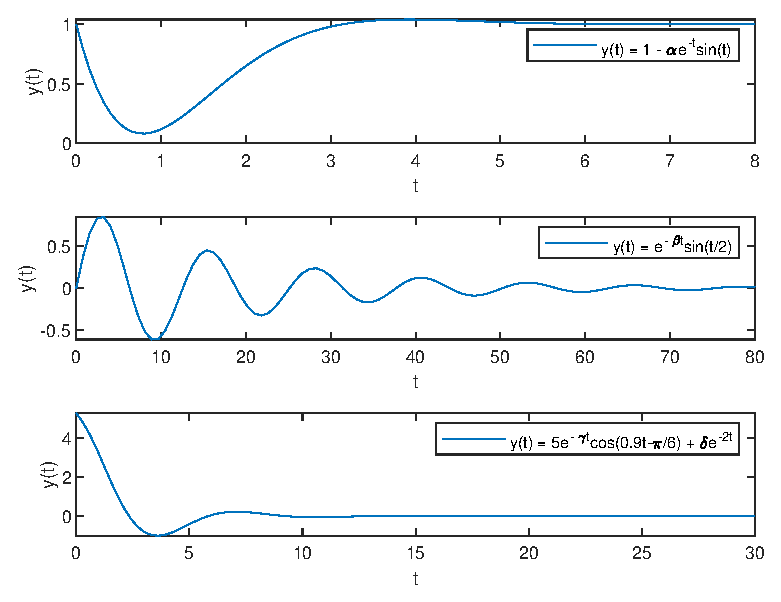
\includegraphics[width=0.8\textwidth]{wykres1.eps}
    \caption{Wykresy funkcji: (a) \(y(t) = 1 - ze^{-t}\sin(t)\), (b) \(y(t) = e^{-\beta t}\sin(\pi t/2)\), (c) \(y(t) = 5e^{-\gamma t}\cos(0.9t - \pi/6) + \delta e^{-2t}\).}
    \label{fig:wykresy}
\end{figure}

\section*{Zadanie 4}

Korzystając z wbudowanych funkcji Matlaba:
\begin{enumerate}
    \item[(a)] wygenerować liczbę \( k \in [1, 10] \) w sposób losowy,
    \item[(b)] zdefiniować liczbę \( a = \) ostatnia cyfra numeru albumu \( + 1 \),
    \item[(c)] dla zdefiniowanych wartości \( k \) i \( a \) wygenerować wykresy funkcji przedstawionych na poniższym rysunku na przedziale \([0, 10\pi]\) (zgodnie z przedstawionym stylem i kolorystyką),
    \item[(d)] podpisać wykresy zgodnie z przykładem.
\end{enumerate}

\begin{lstlisting}

k0 = 1;
k1 = 10;
k = k0 + (k1-k0)*rand;

a = 1 + 1;

x = linspace(0,10*pi,1000);
axis([0 10*pi -1 1]);

y1 = exp(-x/k);
y2 = -exp(-x/k);
y3 = exp(-x/k).*sin(a*x);

figure;
plot(x,y1,'--k','linewidth',2);
axis([0 10*pi -1 1]);
hold on;
plot(x,y3,'g','linewidth',2);
plot(x,y2,'-.b','linewidth',2);
hold off;

legend(['exp(-x/k)'], ...
       ['exp(-x/k)*sin(ax)'], ...
       ['-exp(-x/k)'], ...
       Location='southeast');

title(['k = ' num2str(k) ', a = ' num2str(a)'']);


\end{lstlisting}

\begin{figure}[h]
    \centering
    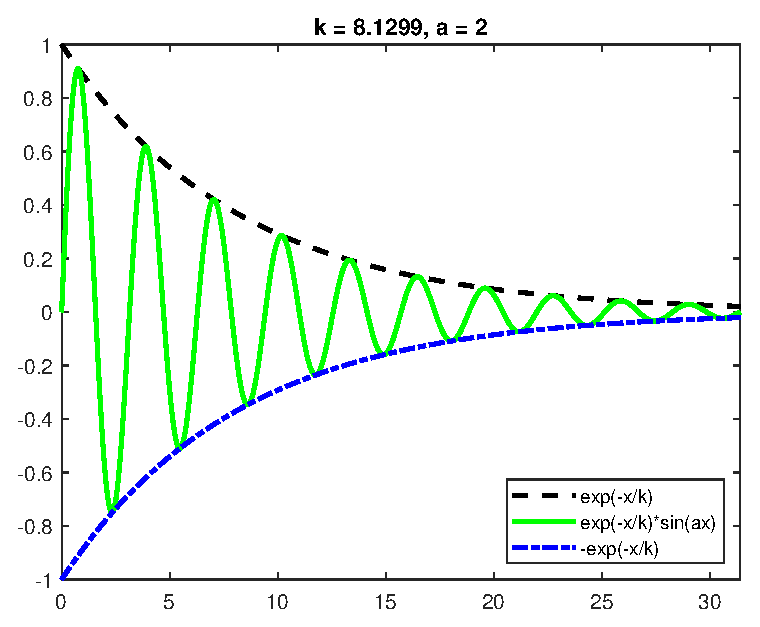
\includegraphics[width=0.8\textwidth]{wykres2.eps}
    \caption{Wykresy funkcji \( y(t) \) dla losowej wartości \( k \) i \( a = \) ostatnia cyfra albumu \( + 1 \).}
    \label{fig:wykresy}
\end{figure}

\end{document}